%%% In this section, you will describe all of the various artifacts that you will generate and maintain during the project life cycle. Describe the purpose of each item below, how the content will be generated, where it will be stored, how often it will be updated, etc. Replace the default text for each section with your own description. Reword this paragraph as appropriate.

\subsection{Major Documentation Deliverables}

\subsubsection{Project Charter}
A project charter is the statement of scope, objectives and people who are participating in a project. It begins the process of defining the roles and responsibilities of those participants and outlines the objectives and goals of the project. The charter also identifies the main stakeholders and defines the authority of the project manager.
Project Charter for this project is uploaded in overleaf, and it is made available to all the group member and all of them will have access to modify or update any required content with all group approval.  

\subsubsection{System Requirements Specification}
System Requirement Specifications are kept as a doc file and is made available in google doc. All requirements are collected in that doc file and each addition of the requirements is made with group discussions and are prioritized on the basis of functionalities they required and the usefulness of that requirement to make our application more applicable and worthy.

\subsubsection{Architectural Design Specification}
The system is designed using the Object Oriented architectural style. As it provide a high-level overview of how the functionality and responsibilities of the system were partitioned and then assigned to subsystems or components. This document is also  The overall architecture is a Event driven using the React Native framework. The system consists of the Client component, Database component and all set of rules to be executed base of the events created by user and notify the user. 


\subsubsection{Detailed Design Specification}
    Core feature of our application will work as shown below
    \begin{figure}[h!]
        \centering
        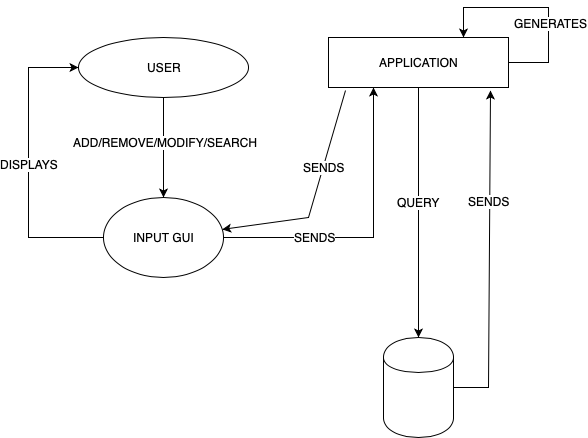
\includegraphics[width=.5\textwidth]{images/core}
        \caption{Informal-Data Flow}
    \end{figure}


\subsection{Recurring Sprint Items}
\subsubsection{Product Backlog}
The product backlog is a kind of living document, as it keeps changing on the basis of the feature being added and the requirement of the system. Each entry on the product backlog as so designed that it will add value for the customer. Product backlog main consist of the  list of all things that needs to be done within the project. It replaces the traditional requirements specification artifacts. Scrum master is responsible for keeping the product backlog up to date with the discussion to the group mate as we are the product owners. We will be using spreed-sheet to maintain the product back log and will be using google doc to share it with all team members. 

\subsubsection{Sprint Planning}
As we have our own system, all the team members will be discussing about the features of the application and all the requirements, and all the sprint goals will be updated in the spreed sheet. A scrum master or coach typically facilitates sprint planning in order to ensure that the discussion is effective and that there is agreement to the sprint goal and that the appropriate product backlog items are included in the sprint backlog. Generally to complete our project our team will required no more that 10-11 sprints.

\subsubsection{Sprint Goal}
Each of the team member is responsible achieve the spring goal. As the scrum master the assigned the task to the individual, its their duty to complete that task in given time frame so that it won't affect other team, who are depend upon the completion of the given task for next phase of sprint cycle. As it is our own product no customer involvement is necessary but as a consumer we will be consulting couple of our friends for feedback on our features implemented in each sprint cycle.  

\subsubsection{Sprint Backlog}
Each meeting will cover the task that are do and the remaining task. All the task are kept in the form of spreadsheet, so its easier for everybody to keep track of the system progress. once all the remaining task is decided, scrum master will be assigning the task to each of the team member including him/her. 

\subsubsection{Task Breakdown}
As we are building our own product, the scrum master will be responsible to divide the task to be completed in that sprint cycle and based on the field of as individual, scrum master will assign the work and s/he will keep the record of assigned task and individual are obliged to give the progress report on the daily basic to the scrum master.


\subsubsection{Sprint Burn Down Charts}
On each sprint cycle one of the group member is assigned as a team leader(scrum master) who will note down every progress report of all team members and s/he will be responsible to make the sprint burn down chart based on the assigned work to the team members and due dates. As each task will assigned certain points,i.e harder the task more points it carries and individual will report his/her daily progress to the team leader and based on that team leader will generate the excel chart to generate the burn down chart for each sprint. As all the materials is made available in google doc, if some mistakes are done by anybody, other group member can correct it.  

                   \begin{figure}[!h]
                        \centering
                        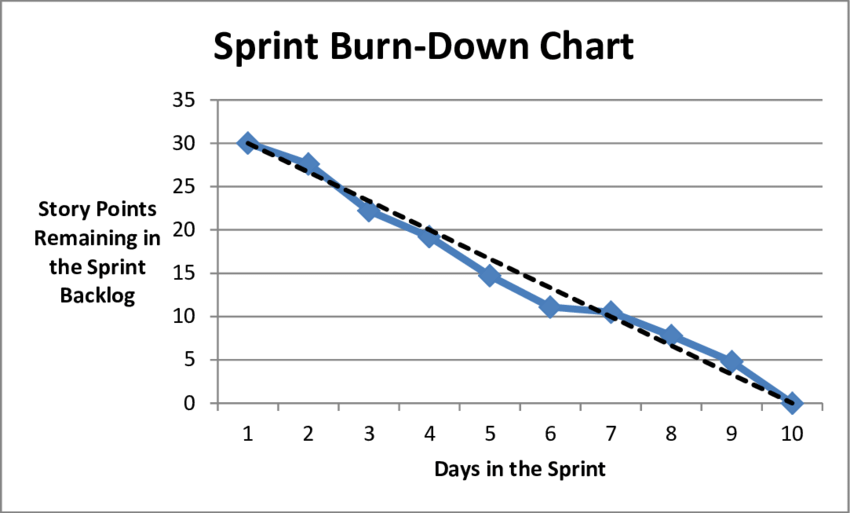
\includegraphics[width=0.5\textwidth]{images/burn}
                        \caption{Example sprint burn down chart \cite{Anon2019}}
                    \end{figure}
                   

\subsubsection{Sprint Retrospective}
Our every team discussion are written in our ENB with exact time and date, title of discussions, ideas created, decisions taken and reasons of selection of that specific decision. So if any of us wants to look back about why we took that decision can refer to ENB. Even though our ENB will be individual, almost all the content inside will be similar because every suggestions and things will be noted there, regardless whose opinion is that. This note taking process continues as our meeting starts and will end after couple aof minutes after meeting ends in order to give individual to note down the missing part from the peers. 


\subsubsection{Individual Status Reports}
On each sprint meeting each member will be assigned task to do with the due dates, and our team leader at that specific time will responsible to keep track of everyone in the team and keep record of quality of result produced by the team member in that given specific time. At the end of each sprint cycle team leader is responsible to submit the individual status report to the professor in-order to give the picture about how team is doing.


\subsubsection{Engineering Notebooks}
Engineering Notebooks is one of the efficient, easy way of keeping track of progress and counted as the legal form, if any legal issue occurs. So we will be updating our notebook on every meeting, and truly the number of pages will depend upon the ideas, each of the team member comes up with. Our ENB will be signed as a "witness" by our professor.   


\subsection{Closeout Materials}


\subsubsection{System Prototype}
Basically our final project is the full functioning mobile application. So we will allow any user to do testing on their phone and more than happy to get feedback for the improvement. We will be demonstrating our final project early fall 2019. 


\subsubsection{Web Page}
Out project web page will include the introduction to our application, its all of the features. Our targeted consumer, all the developers name with their linked profile. And we will keep updating our application as the requirements increases and will announce all the releases in the web page.


\subsubsection{Demo Video}
In our demo we will be using a well functioning application from our phone to do various task which include its core features. Our demo might takes about 8-10 minutes.


\subsubsection{Source Code}
All of our team members are familiar with GitHub and had done several project using it as a version control system, we had decided to use it as our version control tool. All the repository created will be private and no source code will be provide to the customer. As we planed to deploy out final application to the apple store, its free to use for public. All out license term and condition will be listed in a single readme file.


\subsubsection{Source Code Documentation}
Almost all  of the documentation are generated using latex and we will be using overleaf as a leTex editor, our final documentation will be provided in PDF format



\subsubsection{Installation Scripts}
Once our application is deployed in the app store, user will be able to search the app from their play store on their and can install it for free of cost.

\subsubsection{User Manual}
User will be have access to click the help option from the menu bar in the application itself, which will teach the steps to be able to use the various feature of the application.
